%!TEX root = BA-Bauer.tex

\subsection{STMicroelectronics CubeMX}
Die Firma STMicroelectronics\textsuperscript{®} bietet für Programmierung der eigenen MCUs und Mikroprozessoren eine Reihe von kostenloser Software zum Download an. Darunter befindet sich die Software CubeMX, die für jeden MCU und jedes Entwicklungsboard von STMicroelecronics\textsuperscript{®} verwendet werden kann. Mit der Software können Schnittstellen, Ein und Ausgangspins, Einstellungen der Taktgebung und vieles mehr in einer grafischen Benutzeroberfläche vor der eigentlichen Programmierung konfiguriert werden. Dies macht das Durchsuchen des Handbuchs nach den entsprechenden Registern überflüssig. CubeMX generiert $.c$ und $.h$ Dateien mit diversen Funktionen für die konfigurierten Schnittstellen und die Hardware. 
Abbildung \ref{fig:CubeMXClock} zeigt die Benutzeroberfläche zur Konfiguration der Taktgebung in CubeMX. 
\begin{figure}[h]
	\centering
	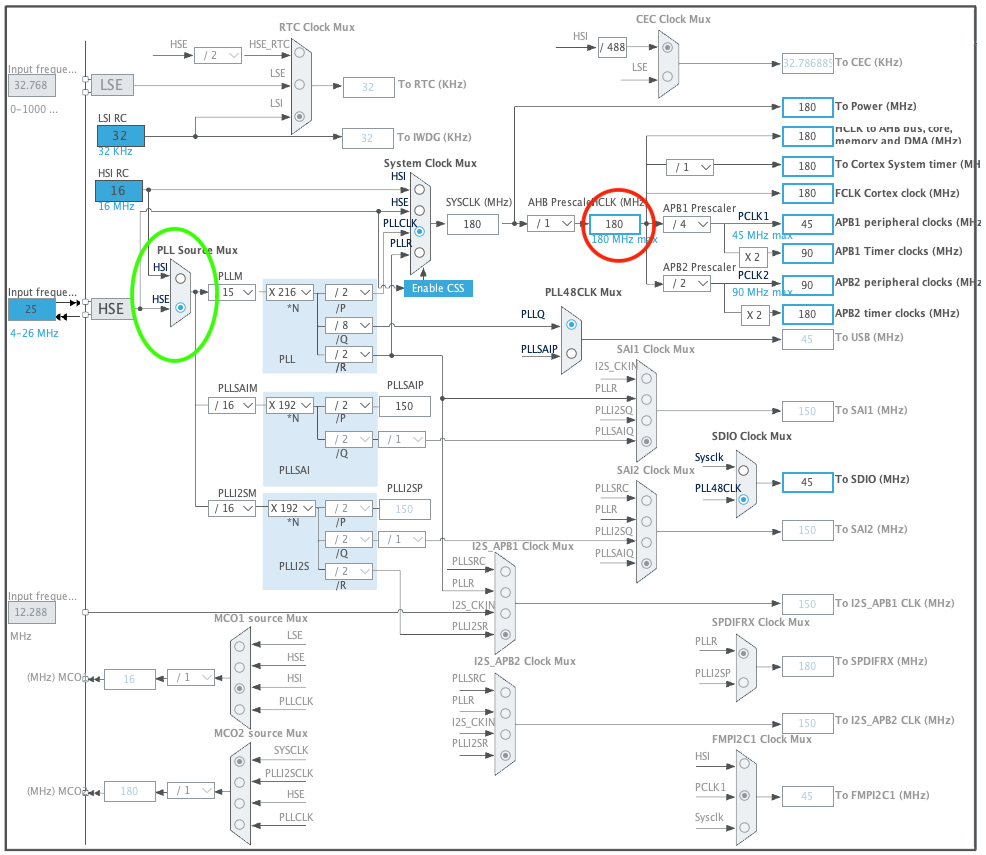
\includegraphics[width=.5\linewidth]{CubeMX-clock-mark}
	\caption{CubeMX Clock Configuration}
	\label{fig:CubeMXClock}
\end{figure}
Die Oberfläche ist nach der Flussrichtung der Taktsignale durch die Parameter und Umschalter angeordnet. Auf der linken Seite finden sich die Oszillatoren, deren Frequenz durch die in der Mitte befindlichen Parameter und Umschalter geteilt oder multipliziert werden kann. Auf der rechten Seite befinden sich die ausgehenden Taktfrequenzen für die einzelnen Schnittstellen. Um den $HSE$-Oszillator zu verwenden, wird im grün markierten Bereich der $HSE$-Umschalter aktiviert und die Frequenz des Oszillators links neben dem grün markierten Bereich eingeben. Damit der MCU mit der maximalen Taktfrequenz von 180\,MHz arbeitet, wird das rot markierte Feld mit 180 beschrieben. Die Parameter und Umschalter, die zum Erreichen der gewählten Taktfrequenz der MCU und der verwendeten Schnittstellen nötig sind, werden von CubeMX berechnet. Wegen der großen Anzahl an Parametern ist das richtige Einstellen der Taktfrequenzen per Hand mit sehr großem Aufwand verbunden. CubeMX unterstützt den Prozess des Programmierens auch in der Konfiguration von Schnittstellen. Der in dieser Arbeit verwendete STM32F446ZE MCU besitzt 20 Schnittstellen, welche ohne CubeMX einzeln durch das Beschreiben von Registern konfiguriert werden müssten. Mit CubeMX können diese Schnittstellen mithilfe einer grafischen Oberfläche eingestellt werden. Zudem schlägt die Software verwendbare Pins zu den jeweiligen Schnittstellen vor, welche durch die Zuweisung an einem virtuellen MCU der Schnittstelle zugeordnet werden können. Die Pins des MCUs besitzen unter Umständen mehrere Funktionen gleichzeitig, können jedoch nur von einer Schnittstelle parallel verwendet werden. Solche Überschneidungen werden von CubeMX erkannt und können manuell durch die Zuweisung eines anderen noch verfügbaren Pins behoben werden.
%\begin{figure}[h] 
%	\centering
%	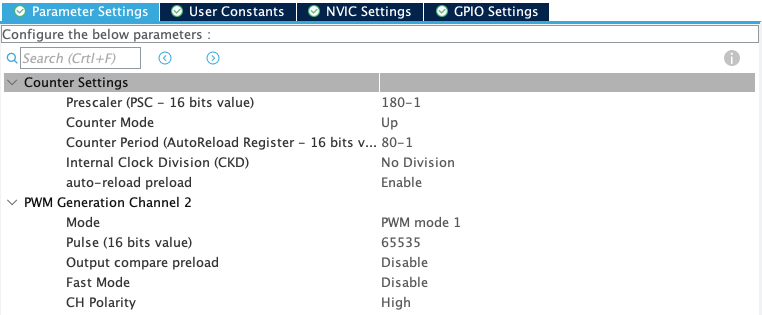
\includegraphics[width=.5\linewidth]{CubeMX-timerconfig}
%	\caption{CubeMX Beispiel Schnittstellenkonfiguration Timer}
%	\label{fig:CubeMXTimer}
%\end{figure}
%Schnittstellenzuweisung der Pins
%Funktionen der Pins
%Interrupts etc. aktivieren
%Koniguration der Schnittstellen
%HAL?!?!